%%
%% This is file `sample-manuscript.tex',
%% generated with the docstrip utility.
%%
%% The original source files were:
%%
%% samples.dtx  (with options: `manuscript')
%% 
%% IMPORTANT NOTICE:
%% 
%% For the copyright see the source file.
%% 
%% Any modified versions of this file must be renamed
%% with new filenames distinct from sample-manuscript.tex.
%% 
%% For distribution of the original source see the terms
%% for copying and modification in the file samples.dtx.
%% 
%% This generated file may be distributed as long as the
%% original source files, as listed above, are part of the
%% same distribution. (The sources need not necessarily be
%% in the same archive or directory.)
%%
%% Commands for TeXCount
%TC:macro \cite [option:text,text]
%TC:macro \citep [option:text,text]
%TC:macro \citet [option:text,text]
%TC:envir table 0 1
%TC:envir table* 0 1
%TC:envir tabular [ignore] word
%TC:envir displaymath 0 word
%TC:envir math 0 word
%TC:envir comment 0 0
%%
%%
%% The first command in your LaTeX source must be the \documentclass command.
%%%% Small single column format, used for CIE, CSUR, DTRAP, JACM, JDIQ, JEA, JERIC, JETC, PACMCGIT, TAAS, TACCESS, TACO, TALG, TALLIP (formerly TALIP), TCPS, TDSCI, TEAC, TECS, TELO, THRI, TIIS, TIOT, TISSEC, TIST, TKDD, TMIS, TOCE, TOCHI, TOCL, TOCS, TOCT, TODAES, TODS, TOIS, TOIT, TOMACS, TOMM (formerly TOMCCAP), TOMPECS, TOMS, TOPC, TOPLAS, TOPS, TOS, TOSEM, TOSN, TQC, TRETS, TSAS, TSC, TSLP, TWEB.
% \documentclass[acmsmall]{acmart}

%%%% Large single column format, used for IMWUT, JOCCH, PACMPL, POMACS, TAP, PACMHCI
% \documentclass[acmlarge,screen]{acmart}

%%%% Large double column format, used for TOG
\documentclass[acmtog, authorversion]{acmart}
\usepackage[htt]{hyphenat}
\usepackage{graphicx}
\graphicspath{{images/}}

%%%% Generic manuscript mode, required for submission
%%%% and peer review
%\documentclass[manuscript,screen,review]{acmart}
%% Fonts used in the template cannot be substituted; margin 
%% adjustments are not allowed.
%%
%% \BibTeX command to typeset BibTeX logo in the docs
\AtBeginDocument{%
  \providecommand\BibTeX{{%
    \normalfont B\kern-0.5em{\scshape i\kern-0.25em b}\kern-0.8em\TeX}}}

%% Rights management information.  This information is sent to you
%% when you complete the rights form.  These commands have SAMPLE
%% values in them; it is your responsibility as an author to replace
%% the commands and values with those provided to you when you
%% complete the rights form.

\setcopyright{acmcopyright}
\copyrightyear{2023}
\acmYear{2023}

%% These commands are for a PROCEEDINGS abstract or paper.
\acmConference[TScIT 39]{39$^{th}$ Twente Student Conference on IT}{July 8,
  2023}{Enschede, The Netherlands}
%
%  Uncomment \acmBooktitle if th title of the proceedings is different
%  from ``Proceedings of ...''!
%
%\acmBooktitle{Woodstock '18: ACM Symposium on Neural Gaze Detection,
% June 03--05, 2018, Woodstock, NY} 
%\acmPrice{15.00}
%\acmISBN{978-1-4503-XXXX-X/18/06}


%%
%% Submission ID.
%% Use this when submitting an article to a sponsored event. You'll
%% receive a unique submission ID from the organizers
%% of the event, and this ID should be used as the parameter to this command.
%%\acmSubmissionID{123-A56-BU3}

%%
%% For managing citations, it is recommended to use bibliography
%% files in BibTeX format.
%%
%% You can then either use BibTeX with the ACM-Reference-Format style,
%% or BibLaTeX with the acmnumeric or acmauthoryear sytles, that include
%% support for advanced citation of software artefact from the
%% biblatex-software package, also separately available on CTAN.
%%
%% Look at the sample-*-biblatex.tex files for templates showcasing
%% the biblatex styles.
%%

%%
%% The majority of ACM publications use numbered citations and
%% references.  The command \citestyle{authoryear} switches to the
%% "author year" style.
%%
%% If you are preparing content for an event
%% sponsored by ACM SIGGRAPH, you must use the "author year" style of
%% citations and references.
%% Uncommenting
%% the next command will enable that style.
%%\citestyle{acmauthoryear}

%%
%% end of the preamble, start of the body of the document source.
\begin{document}

%%
%% The "title" command has an optional parameter,
%% allowing the author to define a "short title" to be used in page headers.
\title{Satellite to Radar: Sequence to Sequence Learning for precipitation forecasting}

%%
%% The "author" command and its associated commands are used to define
%% the authors and their affiliations.
%% Of note is the shared affiliation of the first two authors, and the
%% "authornote" and "authornotemark" commands
%% used to denote shared contribution to the research.

\author{Mark Bruderer}
\email{author@student.utwente.nl}
\affiliation{%
  \institution{University of Twente}
  \streetaddress{P.O. Box 217}
  \city{Enschede}
  \country{The Netherlands}
  \postcode{7500AE}
}



%%
%% By default, the full list of authors will be used in the page
%% headers. Often, this list is too long, and will overlap
%% other information printed in the page headers. This command allows
%% the author to define a more concise list
%% of authors' names for this purpose.
\renewcommand{\shortauthors}{Author}

%%
%% The abstract is a short summary of the work to be presented in the
%% article.
\begin{abstract}
  In this paper, we describe the formatting guidelines for ACM SIG Proceedings.
\end{abstract}

%%
%% The code below is generated by the tool at http://dl.acm.org/ccs.cfm
%% Please copy and paste the code instead of the example below.
%%Optional
%%
%%\begin{CCSXML}
%%<ccs2012>
%% <concept>
%%  <concept_id>10010520.10010553.10010562</concept_id>
%%  <concept_desc>Computer systems organization~Embedded systems</concept_desc>
%%  <concept_significance>500</concept_significance>
%% </concept>
%% <concept>
%%  <concept_id>10010520.10010575.10010755</concept_id>
%%  <concept_desc>Computer systems organization~Redundancy</concept_desc>
%%  <concept_significance>300</concept_significance>
%% </concept>
%% <concept>
%%  <concept_id>10010520.10010553.10010554</concept_id>
%%  <concept_desc>Computer systems organization~Robotics</concept_desc>
%%  <concept_significance>100</concept_significance>
%% </concept>
%% <concept>
%%  <concept_id>10003033.10003083.10003095</concept_id>
%%  <concept_desc>Networks~Network reliability</concept_desc>
%%  <concept_significance>100</concept_significance>
%% </concept>
%%</ccs2012>
%%\end{CCSXML}

%%\ccsdesc[500]{Computer systems organization~Embedded systems}
%%\ccsdesc[300]{Computer systems organization~Redundancy}
%%\ccsdesc{Computer systems organization~Robotics}
%%\ccsdesc[100]{Networks~Network reliability}

%%
%% Keywords. The author(s) should pick words that accurately describe
%% the work being presented. Separate the keywords with commas.
\keywords{Keywords are your own designated keywords.}

\settopmatter{printacmref=false}

%% A "teaser" image appears between the author and affiliation
%% information and the body of the document, and typically spans the
%% page.
\begin{teaserfigure}
  \includegraphics*[width=\textwidth, trim= 0in 16.0in 0in 16.0in]{report/Bachelor's Student Conference Proceedings Paper in LaTeX Template/images/storm.jpg}
  \caption{Plane passing through thunderstorm. - Tom Barrett}
  \Description{Enjoying the baseball game from the third-base
  seats. Ichiro Suzuki preparing to bat.}
  \label{fig:teaser}
\end{teaserfigure}

%%
%% This command processes the author and affiliation and title
%% information and builds the first part of the formatted document.
\maketitle

\section{Introduction}
The \textit{proceedings} are the records of the conference. ACM 
hopes to give these conference by-products a single, high-quality
appearance. To do this, we ask that authors follow some simple 
guidelines. In essence, we ask you to make your paper look exactly 
like this document. The easiest way to do this is simply to down-load 
a template and replace the content with your own material.

\section{Page size}
All material on each page should fit within a rectangle centered on 
the page, beginning 2.54 cm (1") from the top of the page and ending 
with 2.54 cm (1") from the bottom.  The right and left margins should be 
1.9 cm (.75").  The text should be in two 8.18 cm columns with a .83 cm 
(.33") gutter. Page format is International A4.

\section{Typeset text}
\subsection{Normal or body text}
Please use a 9-point Times Roman font, or other Roman font with 
serifs, as close as possible in appearance to Times Roman in which 
these guidelines have been set. The goal is to have a 9-point text, 
as you see here. Please use sans-serif or non-proportional fonts 
only for special purposes, such as distinguishing source code text. 
If Times Roman is not available, try the font named Computer Modern
Roman. On a Macintosh, use the font named Times. Right margins 
should be justified, not ragged.

\subsection{Title and authors}
The title (Helvetica 18-point bold), authors' names (Helvetica 
12-point) and affiliations (Helvetica 10-point) run across the full 
width of the page - one column wide. We also recommend an  e-mail 
address (Helvetica 12-point). See the top of this page for three 
addresses. If only one address is needed, center all address text. 
For two addresses, use two centered tabs, and so on.

\subsection{First Page Copyright Notice}
Please leave the Copyright Notice on the first page as it is but 
change the date and the number of the conference, if necessary.

\subsection{Subsequent pages}
For pages other than the first page, start at the top of the page, and 
continue in double-column format.  The two columns on the last page 
should be as close to equal length as possible.

\begin{table}
\centering \caption{Table captions should be placed above the table}
\begin{tabular}{|c|c|c|c|} \hline
\textbf{Graphics} & \textbf{Top} & \textbf{In-between} & \textbf{Bottom}\\ \hline 
Tables&End&Last&First\\ \hline 
Figures&Good&Similar&Very well\\
\hline\end{tabular}
\end{table}

\subsection{References and Citations}
Footnotes should be Times New Roman 9-point, and justified to the 
full width of the column.\footnote{A footnote in 9-point Times New Roman.}

Use the "ACM Reference format" for references - that is, a numbered 
list at the end of the article, ordered alphabetically and formatted 
accordingly. See examples of some typical reference types, in the new 
"ACM Reference format", at the end of this document. Within this 
template, use the style named references for the text. Acceptable 
abbreviations, for journal names, can be found here: 
http://library.caltech.edu/reference/abbreviations/

The references are also in 9 pt., but that section (see Section 7) is 
ragged right. References should be published materials accessible to 
the public. Internal technical reports may be cited only if they are 
easily accessible (i.e. you can give the address to obtain the report 
within your citation) and may be obtained by any reader. Proprietary
information may not be cited. Private communications should be 
acknowledged, not referenced  (e.g., "[Robertson, personal communication]"). 

References should be put in alphabetical order. All citattions need to be completer, including authors/organisation, title of publication, where it is published, and date.

\section{Page Numbering, Headers and Footers}
Do not include headers, footers or page numbers in your submission. 
These will be added when the publications are assembled.

\section{Figures / Captions}
Place Tables/Figures/Images in text as close to the reference as possible 
(See Figure \ref{fig:abc}).  It may extend across both columns. 


\begin{figure}
    \centering
  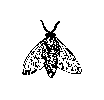
\includegraphics{fly2.eps}
  \caption{Insert caption to place below figure.}
  \label{fig:abc}
\end{figure}

Captions should be Times New Roman 9-point bold.  They should be numbered (e.g., "Table 1" or "Figure 2"), please note that the word for Table and Figure are spelled out. Figure's captions should be centered beneath the image or picture, and Table captions should be centered above the table body.

\section{Sections}
The heading of a section should be in Times New Roman 12-point bold in all-capitals flush left with an additional 6-points of white space above the section head.  Sections and subsequent sub- sections should be numbered and flush left. For a section head and a subsection head together (such as Section 3 and subsection 3.1), use no additional space above the subsection head.

\subsection{Subsections}
The heading of subsections should be in Times New Roman 12-point bold with only the initial letters capitalized. (Note: For subsections and subsubsections, a word like the or a is not capitalized unless it is the first word of the header.)

\subsubsection{Subsubsections}
The heading for subsubsections should be in Times New Roman 11-point italic with initial letters capitalized and 6-points of white space above the subsubsection head.




\section{Type Changes and Special Characters}
We have already seen several typeface changes in this sample.  You
can indicate italicized words or phrases in your text with the
command \texttt{{\char'134}textit}; emboldening with the command
\texttt{{\char'134}textbf} and typewriter-style (for instance, for
computer code) with \texttt{{\char'134}texttt}.  But remember, you
do not have to indicate typestyle changes when such changes are
part of the \textit{structural} elements of your article; for
instance, the heading of this subsection will be in a sans
serif\footnote{A third footnote, here. Let's make this a rather
short one to see how it looks.} typeface, but that is handled by
the document class file. Take care with the use of\footnote{A
fourth, and last, footnote.} the curly braces in typeface changes;
they mark the beginning and end of the text that is to be in the
different typeface.

You can use whatever symbols, accented characters, or non-English
characters you need anywhere in your document; you can find a
complete list of what is available in the \textit{\LaTeX\ User's
Guide}\cite{Lamport:LaTeX}.

\subsection{Math Equations}
You may want to display math equations in three distinct styles:
inline, numbered or non-numbered display.  Each of the three are
discussed in the next sections.

\subsubsection{Inline (In-text) Equations}
A formula that appears in the running text is called an inline or
in-text formula.  It is produced by the \textbf{math} environment,
which can be invoked with the usual \texttt{{\char'134}begin. .
.{\char'134}end} construction or with the short form \texttt{\$. .
.\$}. You can use any of the symbols and structures, from $\alpha$
to $\omega$, available in \LaTeX\cite{Lamport:LaTeX}; this section
will simply show a few examples of in-text equations in context.
Notice how this equation: \begin{math}\lim_{n\rightarrow
\infty}x=0\end{math}, set here in in-line math style, looks
slightly different when set in display style.  (See next section).

\subsubsection{Display Equations}
A numbered display equation -- one set off by vertical space from
the text and centered horizontally -- is produced by the
\textbf{equation} environment. An unnumbered display equation is
produced by the \textbf{displaymath} environment.

Again, in either environment, you can use any of the symbols and
structures available in \LaTeX; this section will just give a
couple of examples of display equations in context. First,
consider the equation, shown as an inline equation above:
\begin{equation}\lim_{n\rightarrow \infty}x=0\end{equation}
Notice how it is formatted somewhat differently in the
\textbf{displaymath} environment.  Now, we'll enter an unnumbered
equation:
\begin{displaymath}\sum_{i=0}^{\infty} x + 1\end{displaymath}
and follow it with another numbered equation:
\begin{equation}\sum_{i=0}^{\infty}x_i=\int_{0}^{\pi+2} f\end{equation}
just to demonstrate \LaTeX's able handling of numbering.

\subsection{Citations}
Citations to articles \cite{bowman:reasoning, clark:pct,
braams:babel, herlihy:methodology}, conference proceedings
\cite{clark:pct} or books \cite{salas:calculus, Lamport:LaTeX}
listed in the Bibliography section of your article will occur
throughout the text of your article. You should use BibTeX to
automatically produce this bibliography; you simply need to insert
one of several citation commands with a key of the item cited in
the proper location in the \texttt{.tex} file
\cite{Lamport:LaTeX}. The key is a short reference you invent to
uniquely identify each work; in this sample document, the key is
the first author's surname and a word from the title.  This
identifying key is included with each item in the \texttt{.bib}
file for your article.

The details of the construction of the \texttt{.bib} file are
beyond the scope of this sample document, but more information can
be found in the \textit{Author's Guide}, and exhaustive details in
the \textit{\LaTeX\ User's Guide}\cite{Lamport:LaTeX}.

This article shows only the plainest form of the citation command,
using \texttt{{\char'134}cite}. This is what is stipulated in the
SIGS style specifications. No other citation format is endorsed or
supported.

\subsection{Tables}
Because tables cannot be split across pages, the best placement
for them is typically the top of the page nearest their initial
cite.  To ensure this proper ``floating'' placement of tables, use
the environment \textbf{table} to enclose the table's contents and
the table caption.  The contents of the table itself must go in
the \textbf{tabular} environment, to be aligned properly in rows
and columns, with the desired horizontal and vertical rules.
Again, detailed instructions on \textbf{tabular} material is found
in the \textit{\LaTeX\ User's Guide}.

Immediately following this sentence is the point at which Table 1
is included in the input file; compare the placement of the table
here with the table in the printed dvi output of this document.

\begin{table}
\centering \caption{Frequency of Special Characters}
\begin{tabular}{|c|c|l|} \hline
Non-English or Math&Frequency&Comments\\ \hline \O & 1 in 1,000&
For Swedish names\\ \hline $\pi$ & 1 in 5& Common in math\\ \hline
\$ & 4 in 5 & Used in business\\ \hline
$\Psi^2_1$ & 1 in 40,000& Unexplained usage\\
\hline\end{tabular}
\end{table}

To set a wider table, which takes up the whole width of the page's
live area, use the environment \textbf{table*} to enclose the
table's contents and the table caption.  As with a single-column
table, this wide table will ``float" to a location deemed more
desirable. Immediately following this sentence is the point at
which Table 2 is included in the input file; again, it is
instructive to compare the placement of the table here with the
table in the printed dvi output of this document.


\begin{table*}
\centering \caption{Some Typical Commands}
\begin{tabular}{|c|c|l|} \hline
Command&A Number&Comments\\ \hline \texttt{{\char'134}alignauthor}
& 100& Author alignment\\ \hline
\texttt{{\char'134}numberofauthors}& 200& Author enumeration\\
\hline \texttt{{\char'134}table}& 300 & For tables\\ \hline
\texttt{{\char'134}table*}& 400& For wider tables\\
\hline\end{tabular}
\end{table*}
% end the environment with {table*}, NOTE not {table}!

\subsection{Figures}
Like tables, figures cannot be split across pages; the best
placement for them is typically the top or the bottom of the page
nearest their initial cite.  To ensure this proper ``floating''
placement of figures, use the environment \textbf{figure} to
enclose the figure and its caption.

This sample document contains examples of \textbf{.eps} and
\textbf{.ps} files to be displayable with \LaTeX.  More details on
each of these is found in the \textit{Author's Guide}.

\begin{figure}
    \centering
    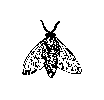
\includegraphics{fly.eps} 
    \caption{A sample black and white graphic (.eps format).}
    \label{fig:fly}
\end{figure}

\begin{figure}
    \centering
    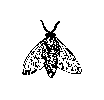
\includegraphics[height=1in, width=1in]{fly.eps} 
    \caption{A sample black and white graphic (.eps format) that has been resized}
    \label{fig:flies}
\end{figure}




As was the case with tables, you may want a figure that spans two
columns.  To do this, and still to ensure proper ``floating''
placement of tables, use the environment \textbf{figure*} to
enclose the figure and its caption.
\begin{figure*}
    \centering 
    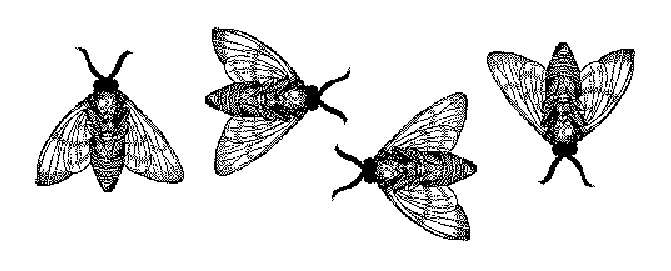
\includegraphics{flies.eps} 
    \caption{A sample black and white graphic (.eps format) that needs to span two columns of text.}
\end{figure*}
and don't forget to end the environment with {figure*}, not
{figure}!


\subsection{Theorem-like Constructs}
Other common constructs that may occur in your article are the
forms for logical constructs like theorems, axioms, corollaries
and proofs.  There are two forms, one produced by the command
\texttt{\textbackslash begin\{theorem\}} and the other by the command
\texttt{\textbackslash begin\{definition\}}; perhaps the clearest and easiest way
to distinguish them is to compare the two in the output of this
sample document:

This uses the \textbf{theorem} environment, created by
the\linebreak\texttt{{\char'134}begin\{theorem\}} command:

\begin{theorem}
Let $f$ be continuous on $[a,b]$.  If $G$ is an antiderivative for
$f$ on $[a,b]$, then
\begin{displaymath}\int^b_af(t)dt = G(b) - G(a).\end{displaymath}
\end{theorem}

The other uses the \textbf{definition} environment, created by the
\texttt{{\char'134}begin\{definition\}} command:
\begin{definition}
If $z$ is irrational, then by $e^z$ we mean the unique number
which has logarithm $z$: \begin{displaymath}{\log e^z =
z}\end{displaymath}
\end{definition}

Two lists of constructs that use one of these forms is given in
the \textit{Author's  Guidelines}.

There is one other similar construct environment, which is already
set up for you; i.e. you must \textit{not} use a
\texttt{{\char'134}newdef} command to create it: the
\textbf{proof} environment.  Here is a example of its use:
\begin{proof}
Suppose on the contrary there exists a real number $L$ such that
\begin{displaymath}
\lim_{x\rightarrow\infty} \frac{f(x)}{g(x)} = L.
\end{displaymath}
Then
\begin{displaymath}
l=\lim_{x\rightarrow c} f(x) = \lim_{x\rightarrow c} \left[ g{x}
\cdot \frac{f(x)}{g(x)} \right ] = \lim_{x\rightarrow c} g(x)
\cdot \lim_{x\rightarrow c} \frac{f(x)}{g(x)} = 0\cdot L = 0,
\end{displaymath}
which contradicts our assumption that $l\neq 0$.
\end{proof}

Complete rules about using these environments and using the two
different creation commands are in the \textit{Author's Guide};
please consult it for more detailed instructions.  If you need to
use another construct, not listed therein, which you want to have
the same formatting as the Theorem or the
Definition\cite{salas:calculus} shown above, use the
\texttt{{\char'134}newtheorem} or the \texttt{{\char'134}newdef}
command, respectively, to create it.

\subsection*{A Caveatfor the \TeX\ Expert}
Because you have just been given permission to use the
\texttt{{\char'134}newdef} command to create a new form, you might
think you can use \TeX's \texttt{{\char'134}def} to create a new
command: \textit{Please refrain from doing this!} Remember that
your \LaTeX\ source code is primarily intended to create
camera-ready copy, but may be converted to other forms -- e.g.
HTML. If you inadvertently omit some or all of the
\texttt{{\char'134}def}s recompilation will be, to say the least,
problematic.

\section{Conclusions}
This paragraph will end the body of this sample document. Remember
that you might still have Acknowledgments or Appendices; brief
samples of these follow.  There is still the Bibliography to deal
with; and we will make a disclaimer about that here: with the
exception of the reference to the \LaTeX\ book, the citations in
this paper are to articles which have nothing to do with the
present subject and are used as examples only.



%%
%% The acknowledgments section is defined using the "acks" environment
%% (and NOT an unnumbered section). This ensures the proper
%% identification of the section in the article metadata, and the
%% consistent spelling of the heading.
\begin{acks}
This section is optional; it is a location for you to acknowledge
grants, funding, editing assistance and what have you.  In the
present case, for example, the authors would like to thank Gerald
Murray of ACM for his help in codifying this \textit{Author's
Guide} and the \textbf{.cls} and \textbf{.tex} files that it
describes.
\end{acks}

%%
%% The next two lines define the bibliography style to be used, and
%% the bibliography file.
\bibliographystyle{ACM-Reference-Format}
\bibliography{sample-base}

%%
%% If your work has an appendix, this is the place to put it.
\appendix
%Appendix A
\section{Headings in Appendices}
The rules about hierarchical headings discussed above for the body
of the article are different in the appendices. In the
\textbf{appendix} environment, the command \textbf{section} is
used to indicate the start of each Appendix, with alphabetic order
designation (i.e. the first is A, the second B, etc.) and a title
(if you include one).  So, if you need hierarchical structure
\textit{within} an Appendix, start with \textbf{subsection} as the
highest level. Here is an outline of the body of this document in
Appendix-appropriate form:
\subsection{Appendix A.1}
Sample text.
\subsection{Appendix A.2}
Sample text.
\subsubsection{Appendix A.2.1}
Sample text.

\paragraph{Inline (In-text) Equations}
\
% This next section command marks the start of
% Appendix B, and does not continue the present hierarchy
\section{Appendix B}
Sample text.
%\balancecolumns % GM June 2007
% That's all folks!


\end{document}
\endinput
%%
%% End of file `sample-authordraft.tex'.
